\documentclass[aspectratio=169,10pt]{beamer}
\usepackage[T1]{fontenc}
\usepackage{lmodern}
\usepackage{graphicx,booktabs,tabularx,amsmath,mathtools,multicol}
\usepackage{tikz}
\usetikzlibrary{arrows.meta,positioning,shapes.geometric,fit,calc}
\usepackage{ragged2e}
\usepackage{fontawesome5}

% A restrained editorial / research-conference visual system
\definecolor{Ink}{HTML}{172B4D}
\definecolor{Navy}{HTML}{102A43}
\definecolor{Teal}{HTML}{087E8B}
\definecolor{Aqua}{HTML}{DDF3F1}
\definecolor{Paper}{HTML}{F7F9FC}
\definecolor{Line}{HTML}{D9E2EC}
\definecolor{Muted}{HTML}{526477}
\definecolor{Amber}{HTML}{D99A24}
\setbeamercolor{normal text}{fg=Ink,bg=white}
\setbeamercolor{structure}{fg=Teal}
\setbeamercolor{frametitle}{fg=Ink,bg=white}
\setbeamercolor{title}{fg=white}
\setbeamercolor{subtitle}{fg=Aqua}
\setbeamercolor{block title}{fg=white,bg=Navy}
\setbeamercolor{block body}{fg=Ink,bg=Paper}
\setbeamercolor{alerted text}{fg=Teal}
\setbeamercolor{itemize item}{fg=Teal}
\setbeamercolor{enumerate item}{fg=Teal}
\setbeamertemplate{navigation symbols}{}
\setbeamertemplate{blocks}[default]
\setbeamertemplate{itemize item}{\raisebox{.15ex}{\tikz\fill[Teal] (0,0) circle (1.15pt);}}
\setbeamertemplate{itemize subitem}{\raisebox{.15ex}{\tikz\fill[Amber] (0,0) circle (.9pt);}}
\setbeamertemplate{enumerate item}{\insertenumlabel.}
\setlength{\leftmargini}{1.35em}
\setlength{\parskip}{1.5pt}
\setlength{\leftmarginii}{1.2em}
\setbeamertemplate{frametitle}{%
  \vspace{3mm}%
  \begin{beamercolorbox}[wd=\paperwidth,ht=8mm,dp=2mm,leftskip=8mm,rightskip=8mm]{frametitle}%
    {\color{Teal}\rule{2.5mm}{2.5mm}}\hspace{2mm}%
    \insertframetitle\hfill{\color{Muted}\scriptsize RESEARCH PRESENTATION}%
  \end{beamercolorbox}%
  \vspace{-1mm}\hspace{8mm}\color{Line}\rule{\dimexpr\paperwidth-16mm\relax}{0.45pt}%
  \vspace{2mm}%
}
\setbeamertemplate{footline}{%
  \leavevmode%
  \hbox{%
  \begin{beamercolorbox}[wd=.78\paperwidth,ht=3.2ex,dp=1.2ex,leftskip=8mm]{author in head/foot}%
    \color{Muted}\scriptsize VOICE-BASED PARKINSON'S DISEASE CLASSIFICATION
  \end{beamercolorbox}%
  \begin{beamercolorbox}[wd=.22\paperwidth,ht=3.2ex,dp=1.2ex,rightskip=8mm plus1fil]{date in head/foot}%
    \color{Teal}\scriptsize \insertframenumber\, / \,\inserttotalframenumber
  \end{beamercolorbox}}%
}
\graphicspath{{assets/}}
\newcommand{\metric}[2]{%
  \begin{beamercolorbox}[sep=8pt,center,wd=\linewidth]{block body}%
    {\color{Teal}\fontsize{23}{25}\selectfont\bfseries #1}\\[-1pt]
    {\color{Muted}\scriptsize #2}%
  \end{beamercolorbox}%
}
\newcommand{\smallcite}[1]{\par\vspace{1mm}{\tiny\color{Muted}#1}}
\title[Voice-based PD classification]{Voice-Based Parkinson's Disease Classification}
\subtitle{Handcrafted Acoustic Features vs. Log-Mel Spectrogram CNN}
\author{Suvinay Foujdar \and Akshat Goyal \and Navya Loshali}
\institute{Department of Computer Science and Engineering\\Bennett University, Greater Noida, India}
\date{Research Project Presentation}

\begin{document}

% 1
{\setbeamercolor{background canvas}{bg=Navy}
\begin{frame}[plain]
\begin{tikzpicture}[remember picture,overlay]
  \fill[Teal] ([xshift=-1.2cm]current page.east) rectangle (current page.south east);
  \fill[Aqua] ([xshift=-2.1cm,yshift=1.4cm]current page.south east) circle (1.05cm);
  \draw[white,opacity=.18,line width=1.1pt] ([xshift=8.1cm,yshift=-1.1cm]current page.north west) .. controls +(1.4,-1.3) and +(-1.4,1.3) .. ([xshift=12.7cm,yshift=-5.9cm]current page.north west);
  \draw[white,opacity=.12,line width=.7pt] ([xshift=8.6cm,yshift=-1.1cm]current page.north west) .. controls +(1.4,-1.3) and +(-1.4,1.3) .. ([xshift=13.2cm,yshift=-5.9cm]current page.north west);
\end{tikzpicture}
\vspace{7mm}
{\color{Aqua}\small\bfseries BENNETT UNIVERSITY  /  RESEARCH PROJECT}\par\vspace{12mm}
{\color{white}\fontsize{31}{36}\selectfont\bfseries Voice-Based Parkinson's\\[-1mm] Disease Classification}\par\vspace{5mm}
{\color{Aqua}\Large Handcrafted Acoustic Features\\and Log-Mel Spectrograms}\par
\vspace{13mm}
{\color{white}\normalsize Suvinay Foujdar  \quad Akshat Goyal  \quad Navya Loshali}\par
\vspace{2mm}{\color{Aqua}\small Department of Computer Science and Engineering\\Greater Noida, India}\par
\vfill
\end{frame}}

% 2
\begin{frame}{Why analyse voice for Parkinson's disease?}
\begin{columns}[T,onlytextwidth]
\column{.56\textwidth}
\begin{itemize}
\item Parkinson's disease can affect phonation, articulation, timing and prosody.
\item Voice recordings offer a non-invasive source of acoustic information.
\item Repeated recordings from the same speaker are correlated.
\item A random recording-level split can leak speaker-specific information into testing.
\end{itemize}
\vspace{2mm}
\begin{block}{Research question}
How do handcrafted acoustic summaries and a Log-Mel CNN compare when evaluation is performed on participants excluded from model development?
\end{block}
\column{.40\textwidth}
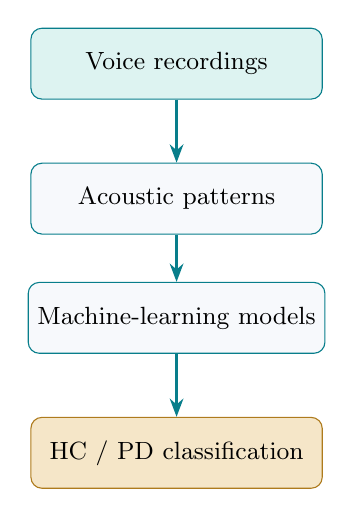
\begin{tikzpicture}[node distance=8mm, every node/.style={rounded corners,align=center,font=\small,minimum width=3.7cm,minimum height=9mm}]
\node[fill=Aqua,draw=Teal] (voice) {Voice recordings};
\node[fill=Paper,draw=Teal,below=of voice] (features) {Acoustic patterns};
\node[fill=Paper,draw=Teal,below=6mm of features] (models) {Machine-learning models};
\node[fill=Amber!25,draw=Amber!80!black,below=of models] (output) {HC / PD classification};
\draw[-{Stealth},thick,Teal] (voice)--(features);
\draw[-{Stealth},thick,Teal] (features)--(models);
\draw[-{Stealth},thick,Teal] (models)--(output);
\end{tikzpicture}
\end{columns}
\end{frame}

% 3
\begin{frame}{Objectives and study contribution}
\begin{columns}[T,onlytextwidth]
\column{.48\textwidth}
\begin{block}{Objectives}
\begin{enumerate}
\item Audit the dataset and participant-folder structure.
\item Build a handcrafted acoustic-feature pipeline.
\item Train and compare four classical classifiers.
\item Build a CNN using five-second Log-Mel inputs.
\item Evaluate both approaches on the same held-out participants.
\end{enumerate}
\end{block}
\column{.48\textwidth}
\begin{block}{What this project contributes}
\begin{itemize}
\item Participant-disjoint evaluation.
\item Recording-level and participant-level reporting.
\item Side-by-side classical ML and CNN implementation.
\item Exploratory permutation-importance analysis.
\end{itemize}
\end{block}
\vspace{2mm}
\centering\small\textcolor{Teal}{Implementation-focused comparison; not a new clinical biomarker.}
\end{columns}
\end{frame}

% 4
\begin{frame}{Dataset: Italian Parkinson's Voice and Speech (IPVS)}\sloppy
\begin{columns}[T,onlytextwidth]
\column{.52\textwidth}
\metric{65}{participants}\vspace{2mm}
\metric{831}{WAV recordings}\vspace{2mm}
\metric{115}{handcrafted feature columns per recording}
\column{.45\textwidth}
\centering
\begin{tabular}{lrr}
\toprule
\textbf{Cohort} & \textbf{People} & \textbf{Recordings}\\
\midrule
Young healthy controls & 15 & 45\\
Elderly healthy controls & 22 & 349\\
Parkinson's disease & 28 & 437\\
\midrule
Total & 65 & 831\\
\bottomrule
\end{tabular}
\vspace{3mm}
\begin{alertblock}{Important cohort detail}
\small The two healthy-control cohorts are combined for binary HC/PD classification, but their original identities are retained during the audit.
\end{alertblock}
\end{columns}
\end{frame}

% 5
\begin{frame}{Dataset audit: verified by the notebook}
\begin{columns}[T,onlytextwidth]
\column{.60\textwidth}
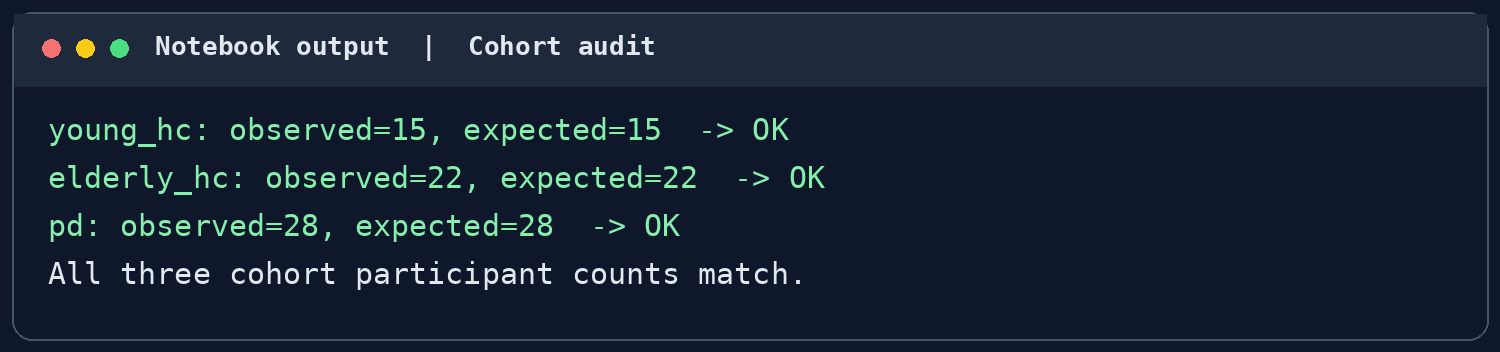
\includegraphics[width=\linewidth,height=.68\textheight,keepaspectratio]{audit_output.png}
\column{.37\textwidth}
\begin{itemize}
\item Cohort counts matched expected folder labels.
\item 65 unique participants identified.
\item 831 feature rows created.
\item 0 feature-extraction errors in the saved run.
\end{itemize}
\begin{block}{Why this matters}
The audit checks the real participant folders before any model is trained. It prevents range folders in the PD directory from being mistaken for participants.
\end{block}
\end{columns}
\smallcite{Evidence: project notebook, cohort audit and feature-table verification cells.}
\end{frame}

% 6
\begin{frame}{End-to-end methodology}
\centering
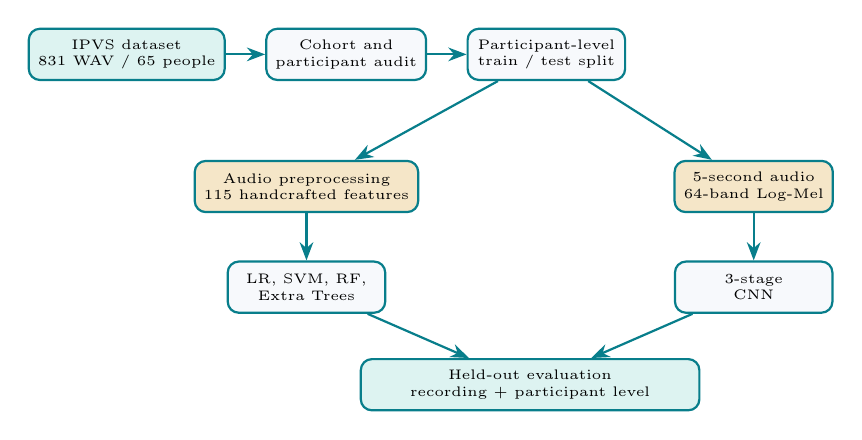
\begin{tikzpicture}[node distance=2mm and 5mm, every node/.style={font=\tiny,align=center,rounded corners,draw=Teal,thick,minimum height=6.5mm,minimum width=2.0cm},arr/.style={-{Stealth},thick,Teal}]
\node[fill=Aqua] (data) {IPVS dataset\\831 WAV / 65 people};
\node[fill=Paper,right=of data] (audit) {Cohort and\\participant audit};
\node[fill=Paper,right=of audit] (split) {Participant-level\\train / test split};
\node[fill=Amber!25,below left=10mm and 6mm of split] (feat) {Audio preprocessing\\115 handcrafted features};
\node[fill=Amber!25,below right=10mm and 6mm of split] (mel) {5-second audio\\64-band Log-Mel};
\node[fill=Paper,below=6mm of feat] (classical) {LR, SVM, RF,\\Extra Trees};
\node[fill=Paper,below=6mm of mel] (cnn) {3-stage\\CNN};
\node[fill=Aqua,below=9mm of $(classical)!0.5!(cnn)$,minimum width=4.3cm] (eval) {Held-out evaluation\\recording + participant level};
\draw[arr] (data)--(audit); \draw[arr] (audit)--(split);
\draw[arr] (split)--(feat); \draw[arr] (split)--(mel);
\draw[arr] (feat)--(classical); \draw[arr] (mel)--(cnn);
\draw[arr] (classical)--(eval); \draw[arr] (cnn)--(eval);
\end{tikzpicture}
\vspace{1mm}
{\small\color{Teal}\bfseries Leakage control:} All recordings from one participant stay in a single partition throughout development and final testing.
\end{frame}

% 7
\begin{frame}{Audio preprocessing and handcrafted features}
\begin{columns}[T,onlytextwidth]
\column{.46\textwidth}
\begin{enumerate}
\item Load WAV and convert stereo to mono.
\item Resample to 16 kHz.
\item Mean-centre and peak-normalise.
\item Extract frame-level acoustic descriptors.
\item Summarise each sequence using mean and standard deviation.
\end{enumerate}
\begin{block}{Feature groups}
20 MFCC + delta-MFCC, spectral centroid, bandwidth, rolloff, zero-crossing rate, RMS, chroma and duration.
\end{block}
\column{.51\textwidth}
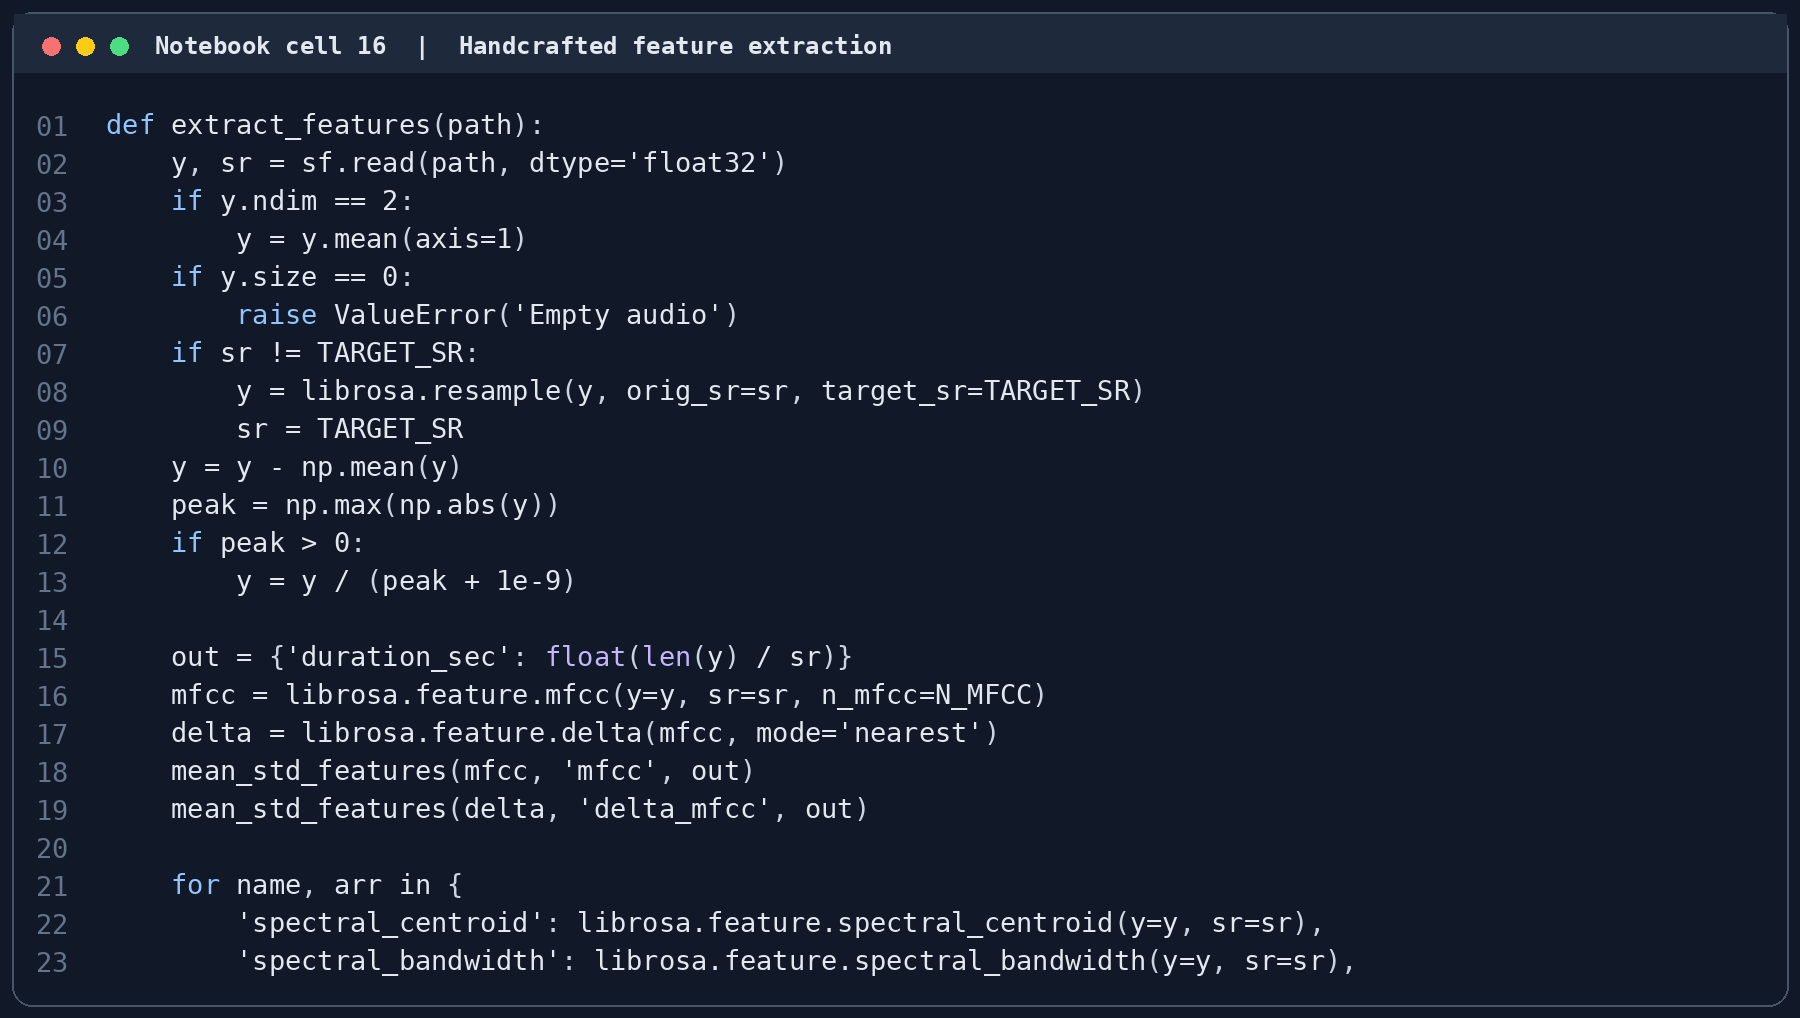
\includegraphics[width=\linewidth,height=.62\textheight,keepaspectratio]{code_features.png}
\end{columns}
\smallcite{Code screenshot: actual feature-extraction function from notebook cell 16 (excerpt).}
\end{frame}

% 8
\begin{frame}{Participant-disjoint split: the key design decision}
\begin{columns}[T,onlytextwidth]
\column{.58\textwidth}
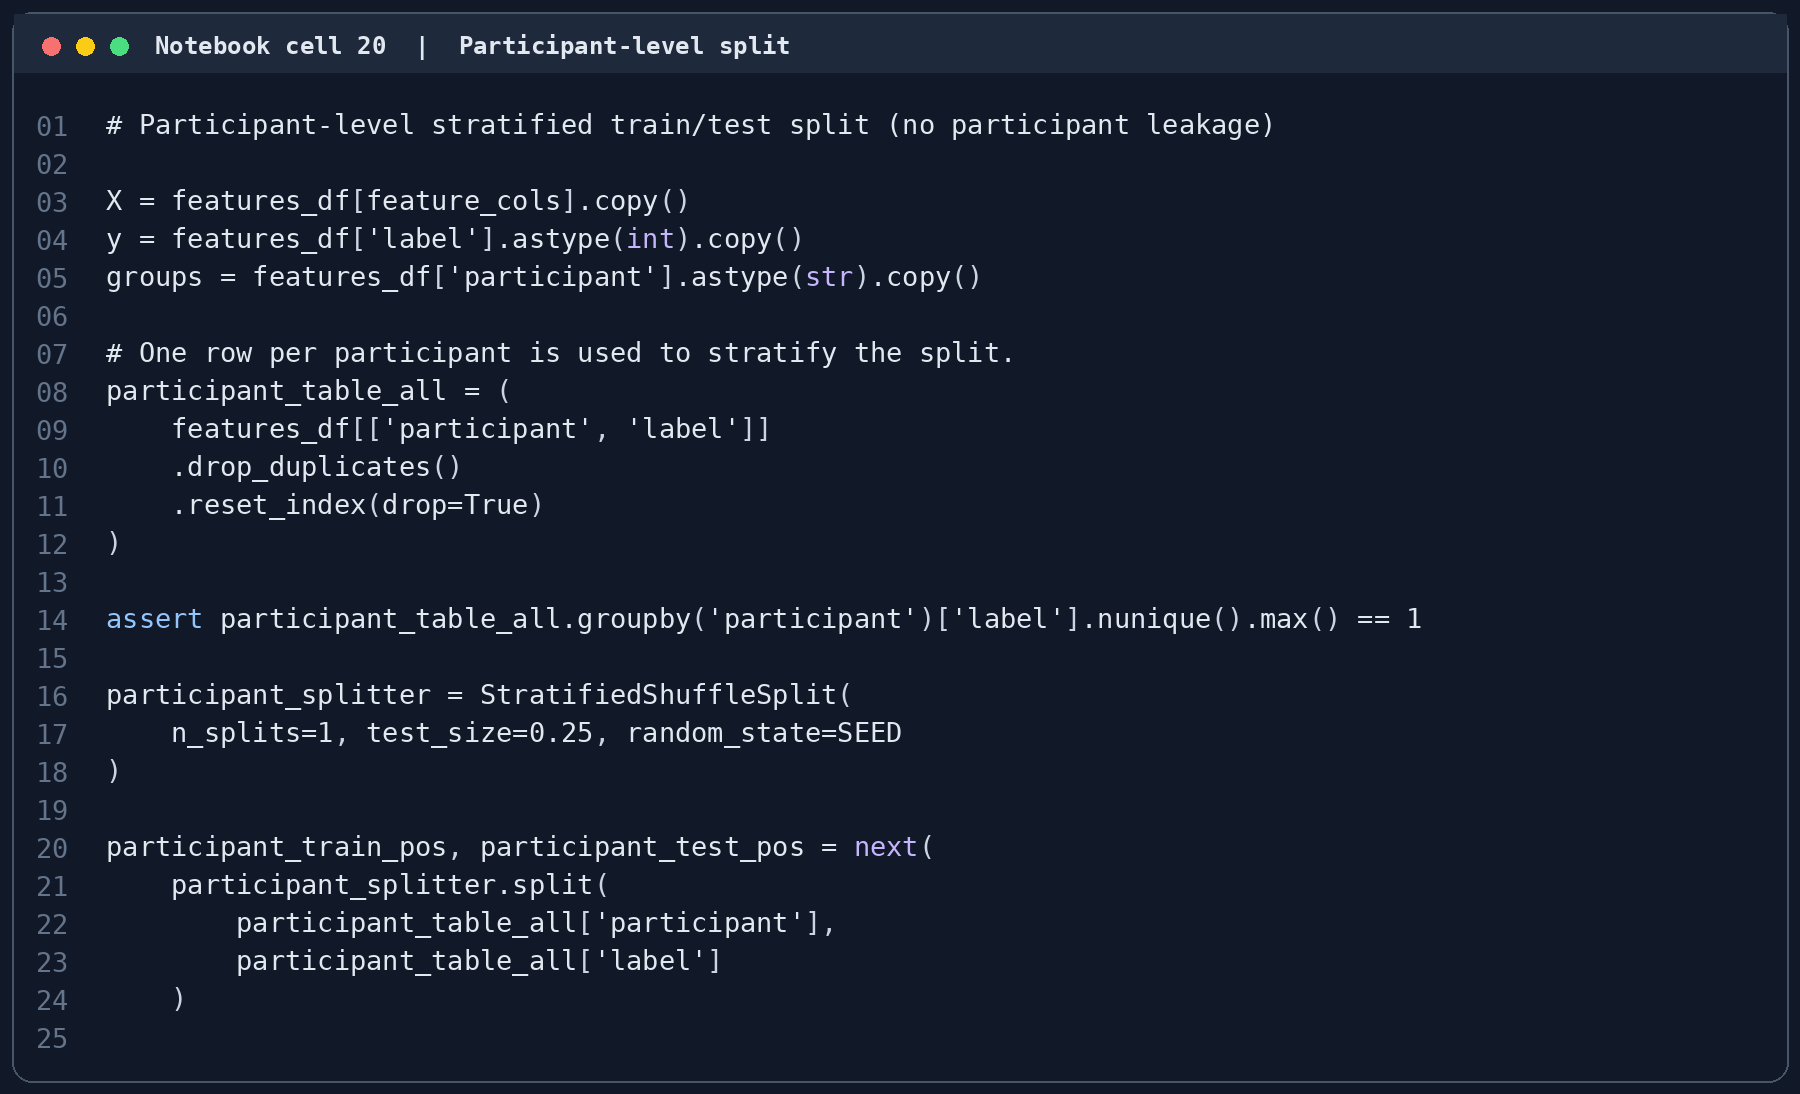
\includegraphics[width=\linewidth,height=.66\textheight,keepaspectratio]{code_split.png}
\column{.38\textwidth}
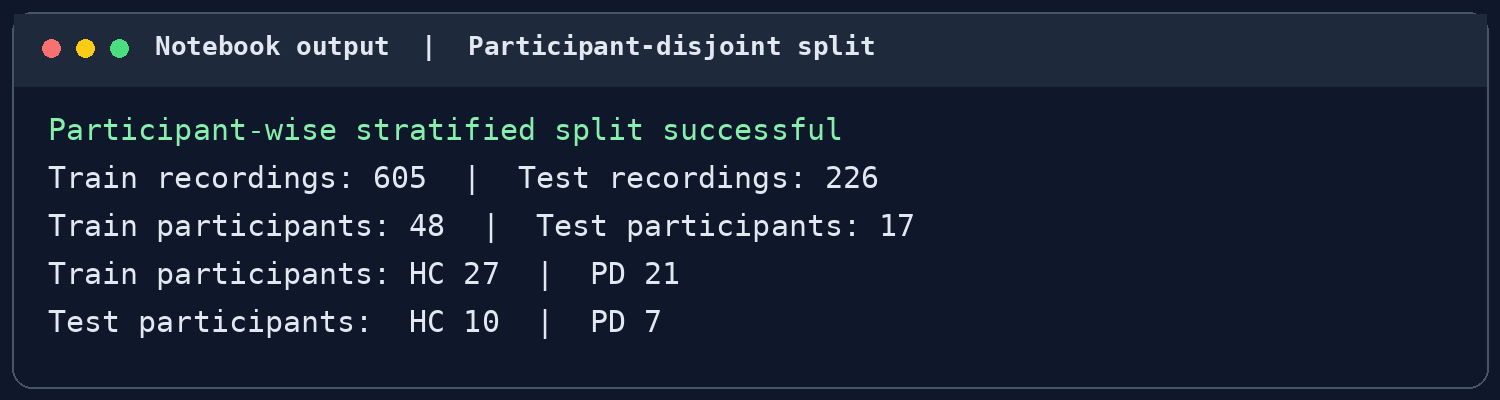
\includegraphics[width=\linewidth,height=.48\textheight,keepaspectratio]{split_output.png}
\begin{block}{Saved split}
\centering
\textbf{48 development people}\\
27 HC + 21 PD\\[1mm]
\textbf{17 held-out people}\\
10 HC + 7 PD
\end{block}
\end{columns}
\smallcite{Code and output: actual notebook cell 20 and its saved execution output.}
\end{frame}

% 9
\begin{frame}{Classical machine-learning comparison}
\begin{columns}[T,onlytextwidth]
\column{.54\textwidth}
\begin{itemize}
\item Logistic Regression
\item RBF-kernel Support Vector Machine
\item Random Forest
\item Extra Trees
\end{itemize}
\vspace{2mm}
Model selection used five-fold participant-stratified cross-validation on the 48 development participants only.
\column{.42\textwidth}
\begin{tabular}{lcc}
\toprule
Model & Mean BA & SD\\
\midrule
RBF-SVM & \textbf{0.9606} & 0.0360\\
Extra Trees & 0.9483 & 0.0474\\
Random Forest & 0.9404 & 0.0469\\
Logistic Reg. & 0.9328 & 0.0302\\
\bottomrule
\end{tabular}
\vspace{3mm}
\begin{alertblock}{Selected model}
RBF-SVM — highest mean balanced accuracy in development cross-validation.
\end{alertblock}
\end{columns}
\end{frame}

% 10
\begin{frame}{CNN: learning from Log-Mel spectrograms}
\begin{columns}[T,onlytextwidth]
\column{.49\textwidth}
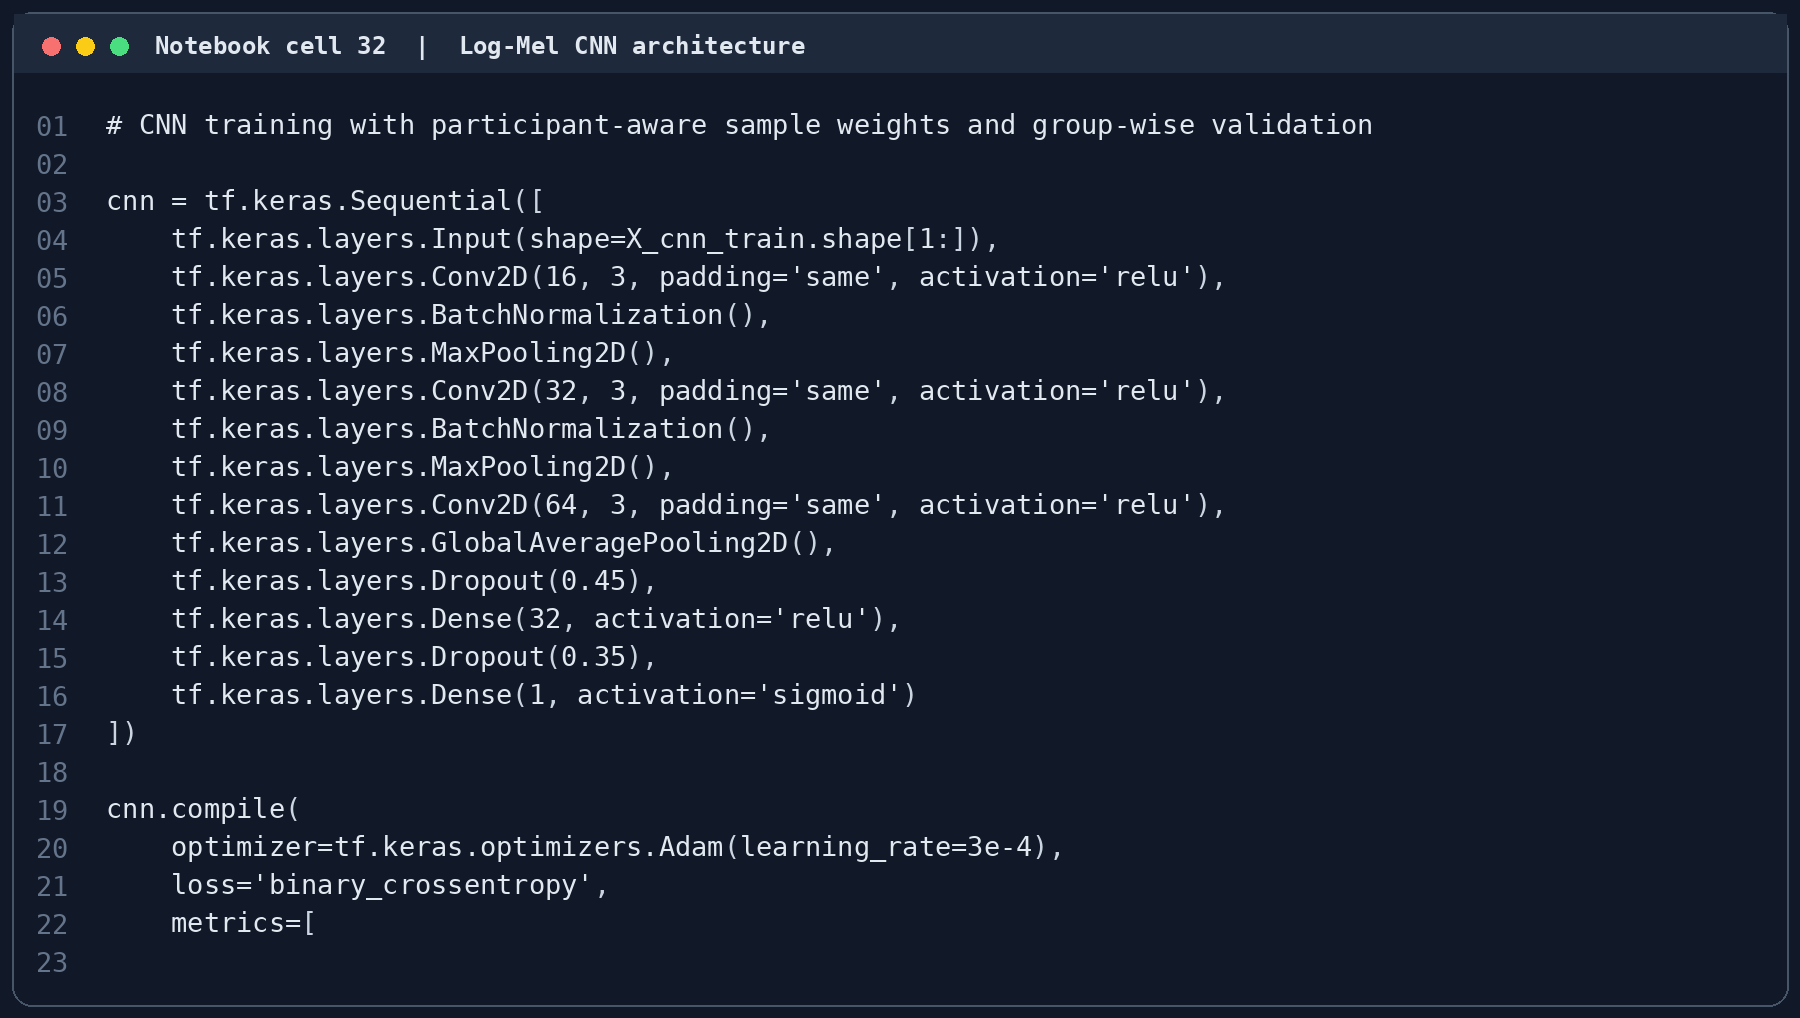
\includegraphics[width=\linewidth,height=.64\textheight,keepaspectratio]{code_cnn.png}
\column{.47\textwidth}
\begin{itemize}
\item Five-second crop from the beginning of each recording.
\item 64 Mel bands; FFT 1024; hop length 256.
\item Input tensor: $64\times313\times1$.
\item Conv2D filters: 16, 32, 64.
\item Batch normalisation, max pooling, global average pooling.
\item Dropout 0.45 / 0.35; Dense 32; sigmoid output.
\end{itemize}
\begin{block}{Training}
Adam ($3\times10^{-4}$), binary cross-entropy, batch size 16, up to 60 epochs, early stopping.
\end{block}
\end{columns}
\smallcite{Code screenshot: actual CNN definition from notebook cell 32 (excerpt).}
\end{frame}

% 11
\begin{frame}{Held-out test results: both levels matter}\sloppy
\begin{columns}[T,onlytextwidth]
\column{.58\textwidth}
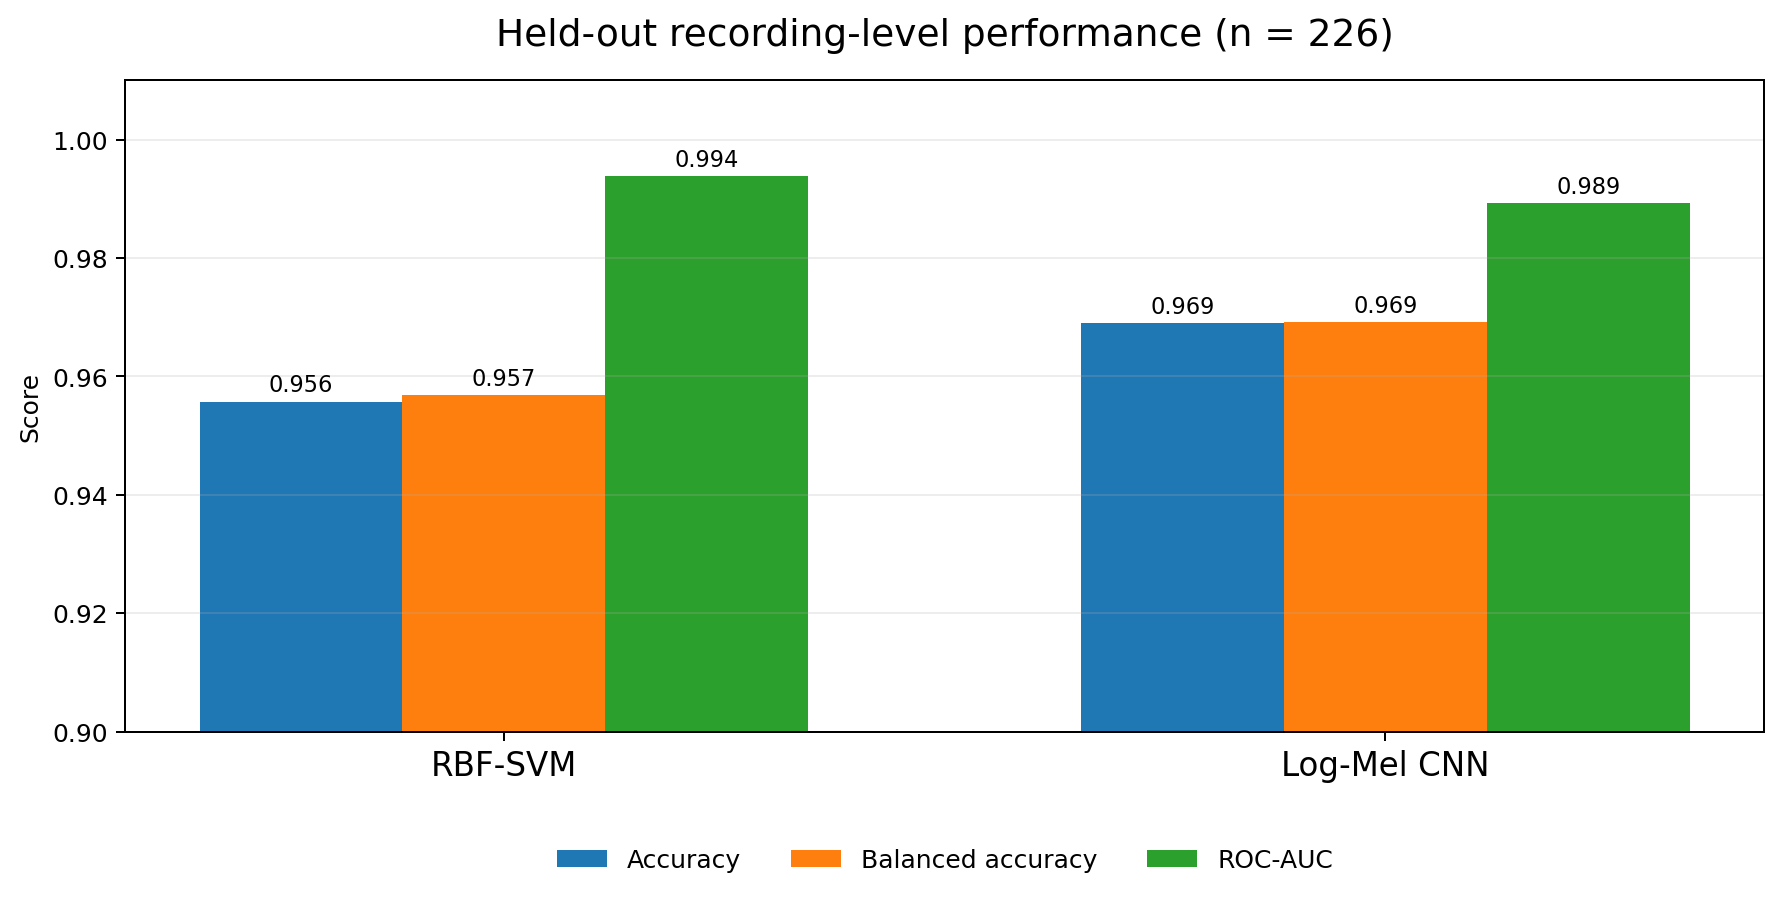
\includegraphics[width=\linewidth,height=.62\textheight,keepaspectratio]{metrics_comparison.png}
\column{.39\textwidth}
\begin{tabular}{lcc}
\toprule
& SVM & CNN\\
\midrule
Recording accuracy & .9558 & \textbf{.9690}\\
Recording BA & .9568 & \textbf{.9692}\\
PD precision & .9358 & \textbf{.9623}\\
PD recall & .9714 & .9714\\
PD F1 & .9533 & \textbf{.9668}\\
ROC-AUC & \textbf{.9939} & .9892\\
\midrule
Participant accuracy & .9412 & .9412\\
Participant BA & .9500 & .9500\\
\bottomrule
\end{tabular}
\end{columns}
\vspace{1mm}
\small\textbf{Test cohort:} 226 recordings from 17 held-out participants. Participant-level metrics are identical in this saved run.
\end{frame}

% 12
\begin{frame}{What did the models get right and wrong?}
\centering
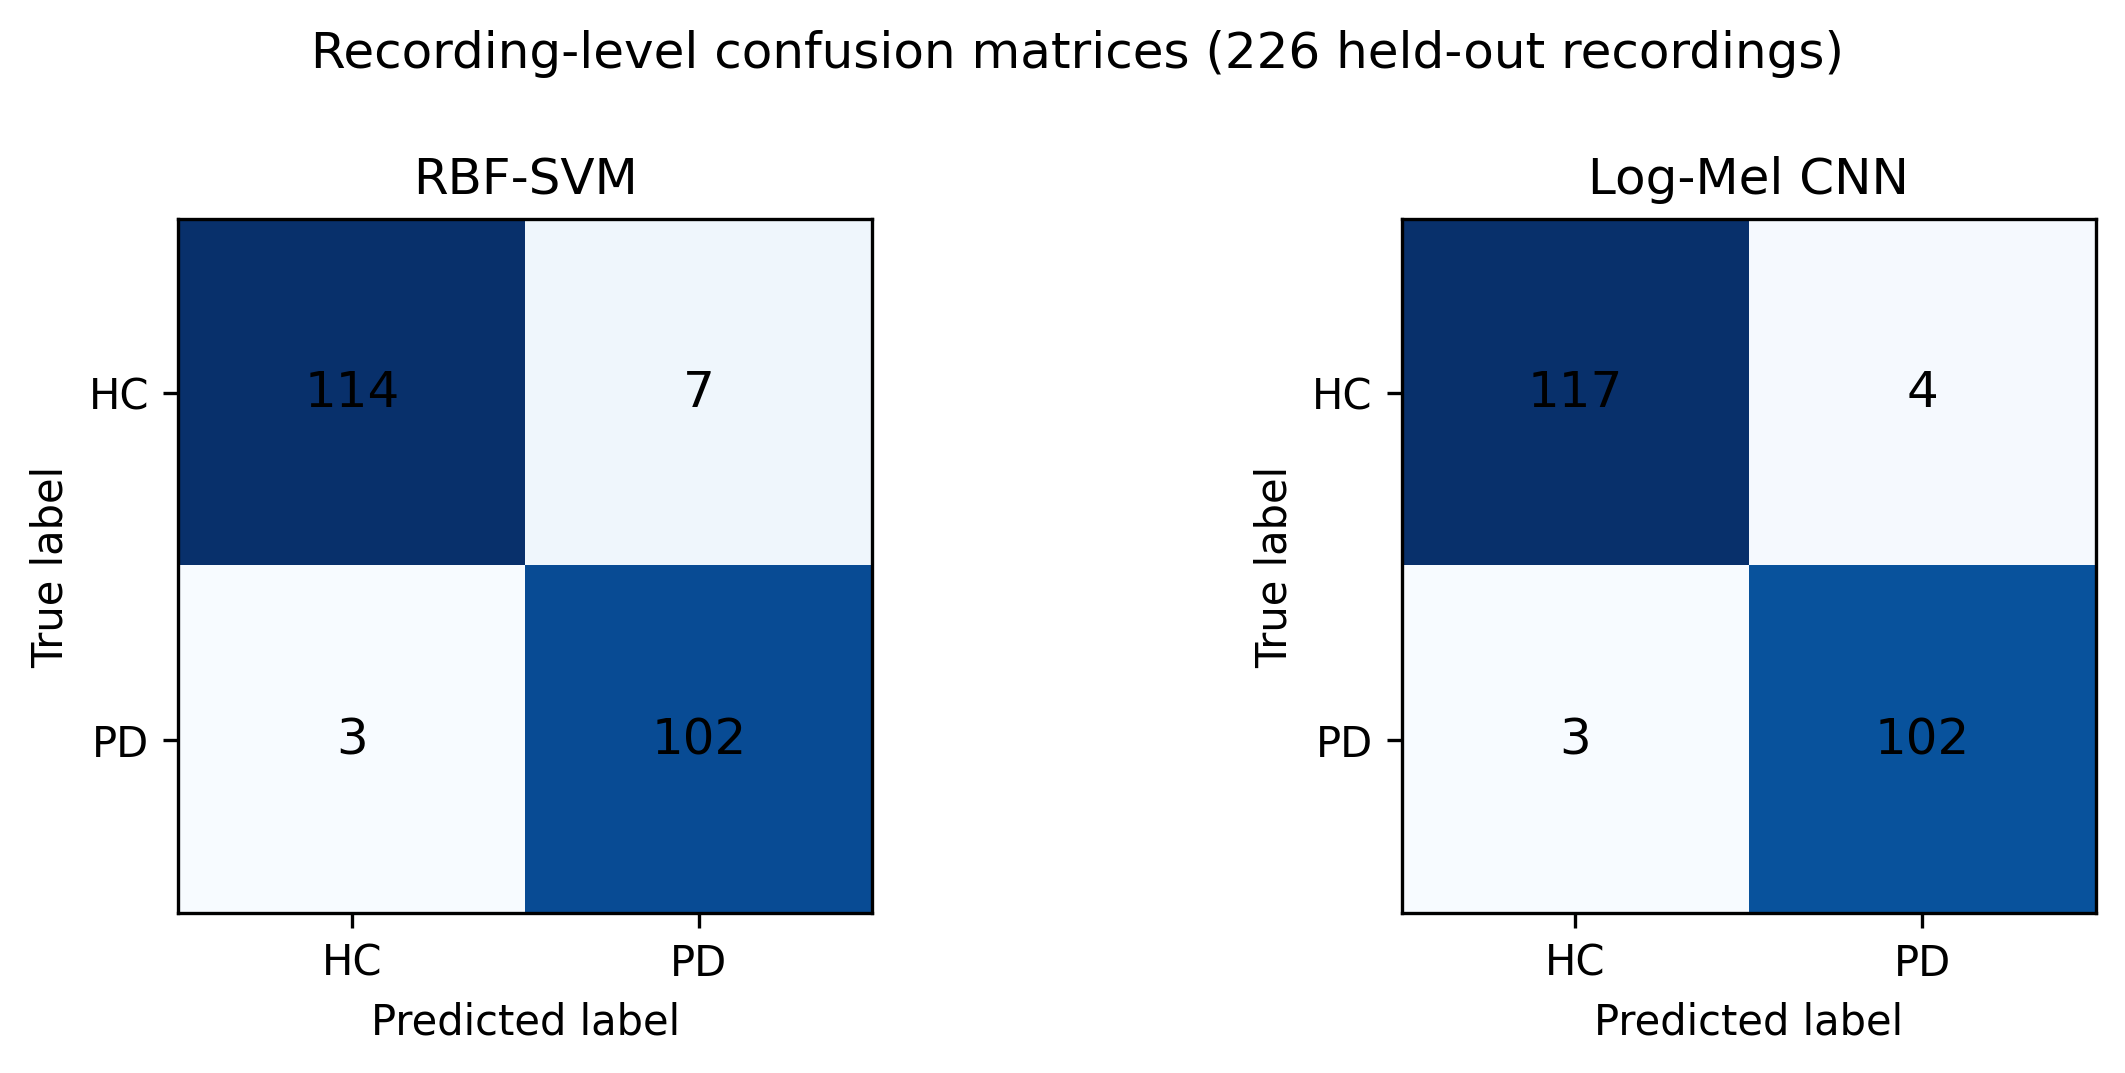
\includegraphics[width=.76\linewidth,height=.55\textheight,keepaspectratio]{recording_confusion_matrices.png}
\vspace{1mm}
\begin{minipage}{.92\linewidth}\centering\small
\textbf{SVM:} 114 HC and 102 PD correct; 7 HC and 3 PD misclassified.\\
\textbf{CNN:} 117 HC and 102 PD correct; 4 HC and 3 PD misclassified.
\end{minipage}
\end{frame}

% 13
\begin{frame}{Exploratory feature importance}
\begin{columns}[T,onlytextwidth]
\column{.62\textwidth}
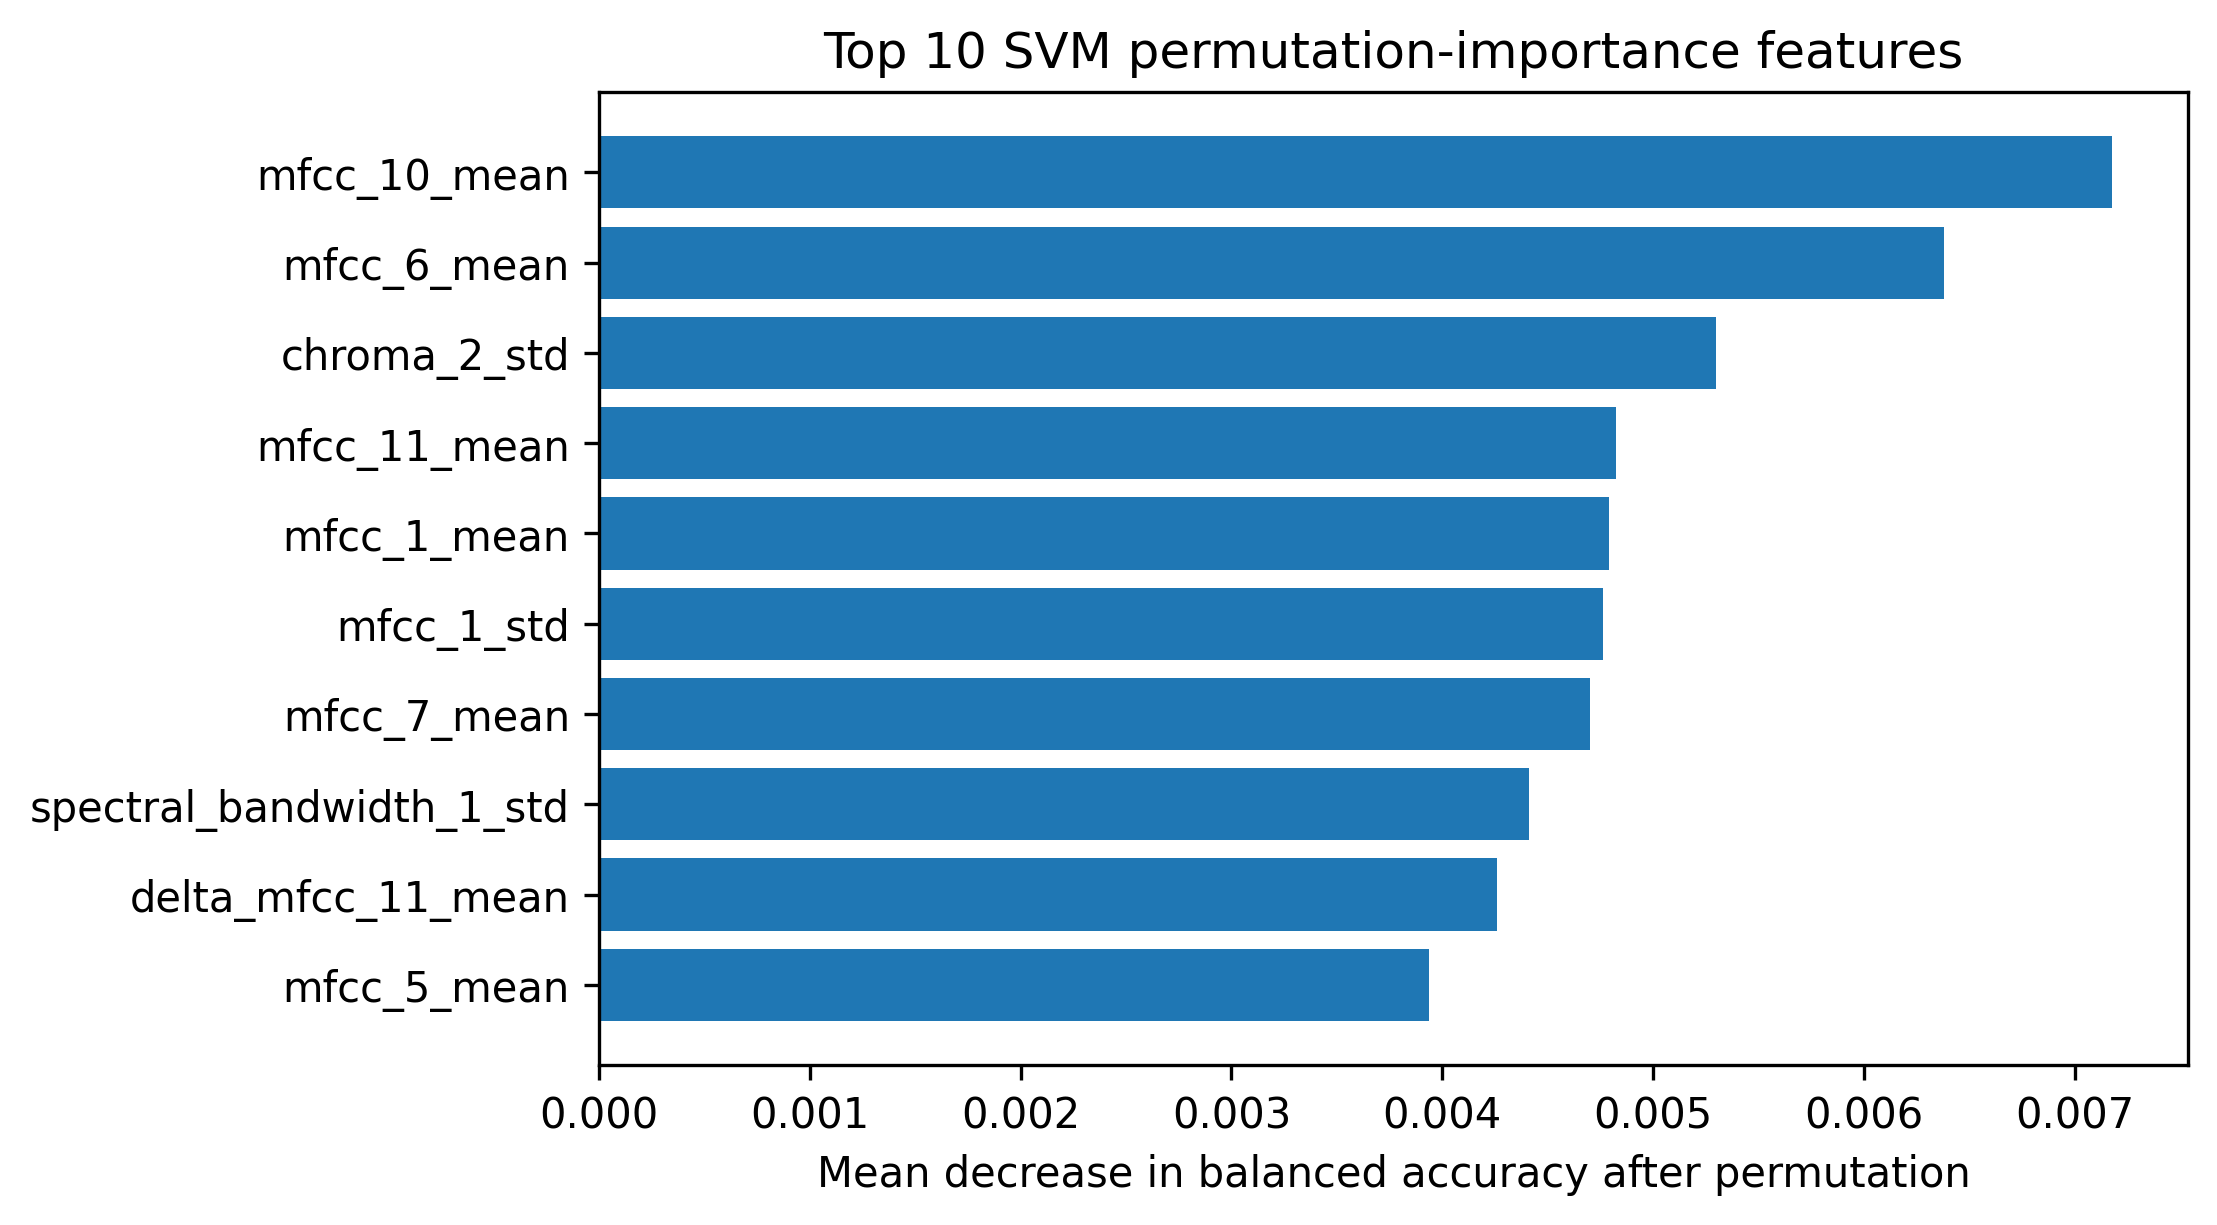
\includegraphics[width=\linewidth,height=.68\textheight,keepaspectratio]{permutation_importance.png}
\column{.34\textwidth}
\begin{itemize}
\item MFCC summary variables appear frequently among top-ranked features.
\item Chroma variability and spectral bandwidth also contribute.
\item Importance is model- and dataset-dependent.
\end{itemize}
\begin{alertblock}{Interpret carefully}
Permutation importance is exploratory; it does not prove causality or identify a clinically validated biomarker.
\end{alertblock}
\end{columns}
\end{frame}

% 14
\begin{frame}{Limitations and future work}
\begin{columns}[T,onlytextwidth]
\column{.48\textwidth}
\begin{block}{Limitations}
\begin{itemize}
\item One dataset and one saved participant split.
\item Only 17 independent held-out participants.
\item HC combines young and elderly cohorts; age effects are not isolated.
\item CNN uses only the first five seconds.
\item No external or prospective clinical validation.
\end{itemize}
\end{block}
\column{.48\textwidth}
\begin{block}{Next steps}
\begin{itemize}
\item Validate on independent datasets and more participants.
\item Repeat grouped outer splits / nested grouped validation.
\item Test segment-selection strategies and recording robustness.
\item Assess calibration and uncertainty.
\item Evaluate prospectively with clinical oversight.
\end{itemize}
\end{block}
\end{columns}
\end{frame}

% 15
\begin{frame}{Conclusion}
\begin{itemize}
\item Implemented two participant-aware pipelines for voice-based HC/PD classification.
\item Handcrafted branch: 115 acoustic summary features; RBF-SVM selected by grouped CV.
\item Deep-learning branch: five-second, 64-band Log-Mel spectrograms processed by a compact CNN.
\item Recording-level accuracy: 95.58\% (SVM) and 96.90\% (CNN).
\item Participant-level accuracy: 94.12\% for both models on 17 held-out people.
\end{itemize}
\vspace{4mm}
\begin{beamercolorbox}[rounded=true,sep=10pt,center]{block body}
\Large\bfseries Participant-aware evaluation shows strong discrimination on the held-out cohort.\\[2mm]
\normalsize Further validation on independent participants and datasets is the next step.\\[2mm]
\normalsize Thank you.\\Questions?
\end{beamercolorbox}
\end{frame}

% 16
\begin{frame}{Selected references}
\footnotesize
\begin{thebibliography}{6}
\bibitem{luna} I. Luna-Ortiz et al., ``Parkinson's Disease Detection from Voice Recordings Using Associative Memories,'' \emph{Healthcare}, vol. 11, no. 11, 1601, 2023.
\bibitem{ngo} Q. C. Ngo et al., ``Computerized analysis of speech and voice for Parkinson's disease: A systematic review,'' \emph{Comput. Methods Programs Biomed.}, vol. 226, 107133, 2022.
\bibitem{amato} F. Amato et al., ``Machine learning- and statistical-based voice analysis of Parkinson's disease patients: A survey,'' \emph{Expert Syst. Appl.}, vol. 219, 119651, 2023.
\bibitem{xavier} D. Xavier et al., ``Voice analysis in Parkinson's disease---a systematic literature review,'' \emph{Artif. Intell. Med.}, vol. 163, 103109, 2025.
\bibitem{malek} H. Sedigh Malekroodi, B.-I. Lee, and M. Yi, ``Voice-Based Detection of Parkinson's Disease Using Machine and Deep Learning Approaches: A Systematic Review,'' \emph{Bioengineering}, vol. 12, no. 11, 1279, 2025.
\bibitem{hossain} M. A. Hossain, E. Traini, and F. Amenta, ``Identification of Parkinson's Disease from Native Italian People: Machine Learning Voice Analysis,'' \emph{BioMed}, vol. 6, no. 3, 15, 2026.
\end{thebibliography}
\end{frame}

\end{document}
